\documentclass[a4paper,12pt]{article}

\usepackage[utf8]{inputenc}
\usepackage[russian]{babel}
\usepackage{graphicx}
\usepackage{enumitem}
\usepackage{hyperref}

\title{Система мониторинга и управления устройствами умного дома}
\date{}

\begin{document}

\maketitle

\section*{Описание}
Система предназначена для мониторинга и управления устройствами умного дома.
Включает \textbf{встраиваемые устройства}, \textbf{сервер/бэкенд} и \textbf{пользовательский интерфейс}.

\section*{Основные функции}

\subsection*{Пользовательский интерфейс}
\begin{itemize}[leftmargin=1.5em]
  \item Графический редактор правил и настроек устройств
  \item Отображение телеметрии с устройств
  \item Магазин устройств
\end{itemize}

\subsection*{Сервер/Бэкенд}
\begin{itemize}[leftmargin=1.5em]
  \item API для пользовательского интерфейса
  \item Модульная система:
        \begin{itemize}
          \item \textbf{Core} + модули (описание устройств и получаемых данных)
        \end{itemize}
\end{itemize}

\subsection*{Хаб}
\begin{itemize}[leftmargin=1.5em]
  \item База данных подключённых устройств
  \item API для связи сервер~$\leftrightarrow$~хаб
\end{itemize}

\subsection*{Устройства}
\begin{itemize}[leftmargin=1.5em]
  \item Подключаются к хабу пользователя
  \item Предоставляют API для отправки телеметрии и управления
\end{itemize}

\section*{Прототип дизайна интерфейса}

\subsection*{Главная страница и показания датчиков}
\begin{center}
  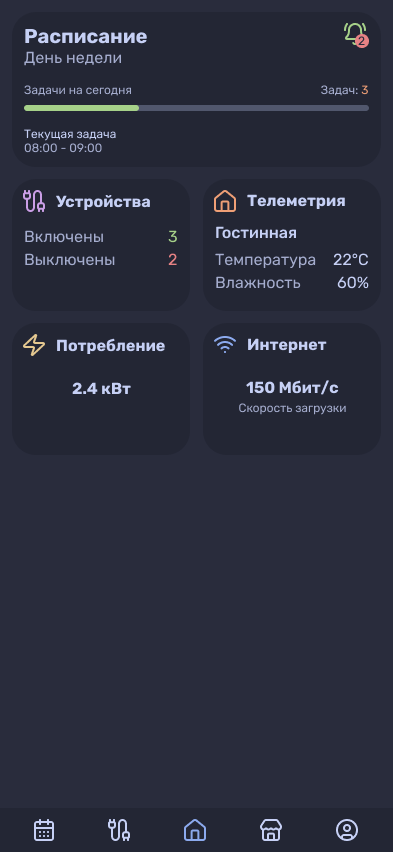
\includegraphics[width=0.425\textwidth]{pics/Main Page.png}
  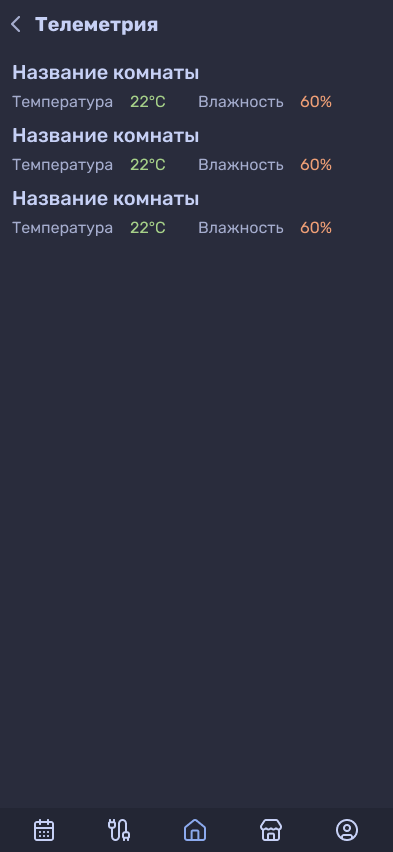
\includegraphics[width=0.425\textwidth]{pics/Telemetry Page.png}
\end{center}

\subsection*{Магазин устройств и карточка товара}
\begin{center}
  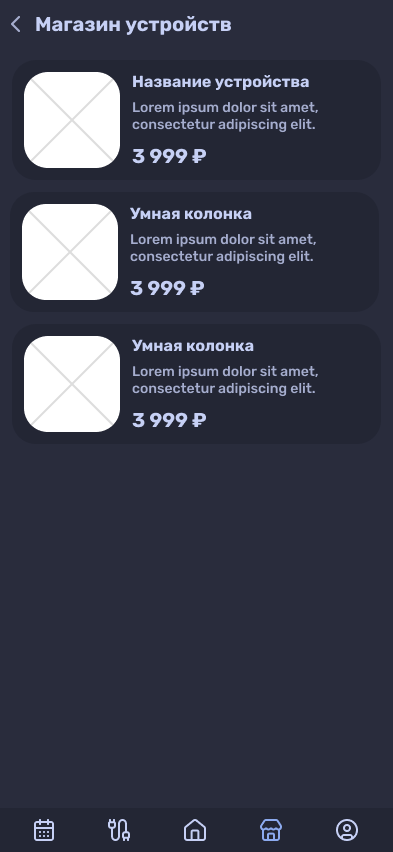
\includegraphics[width=0.425\textwidth]{pics/Store Page.png}
  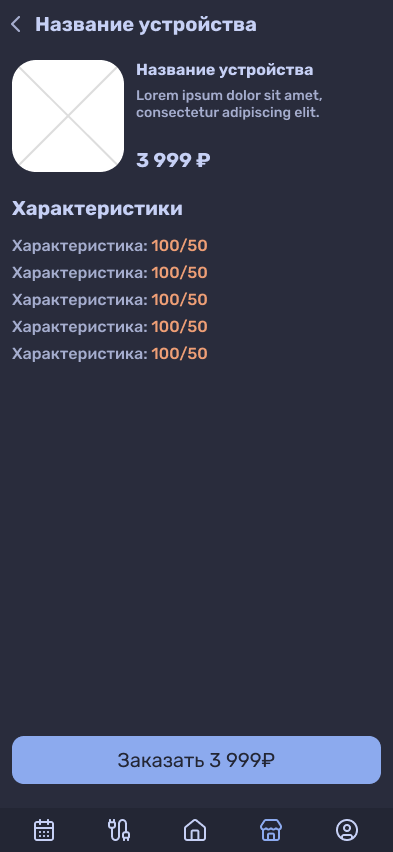
\includegraphics[width=0.425\textwidth]{pics/Single Store Page.png}
\end{center}

\subsection*{Страница устройств и карточка устройства}
\begin{center}
  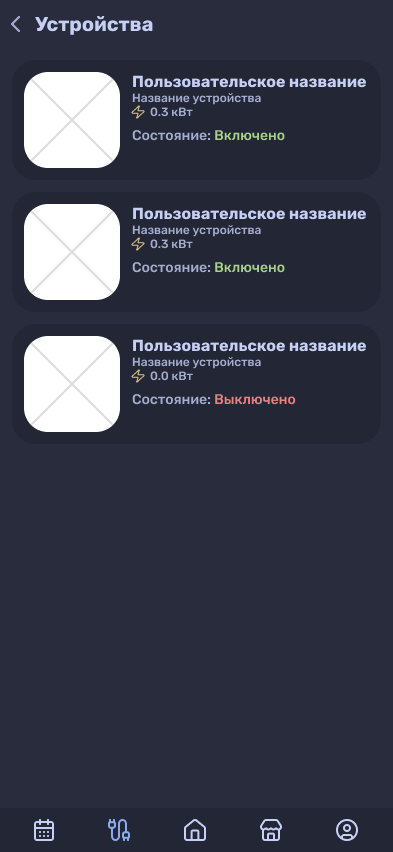
\includegraphics[width=0.425\textwidth]{pics/Devices Page.png}
  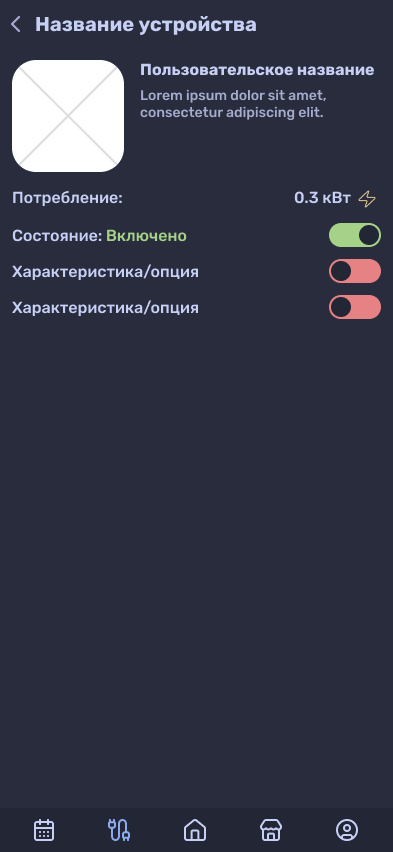
\includegraphics[width=0.425\textwidth]{pics/Single Device Page.png}
\end{center}

\subsection*{Расписание и создание новой задачи}
\begin{center}
  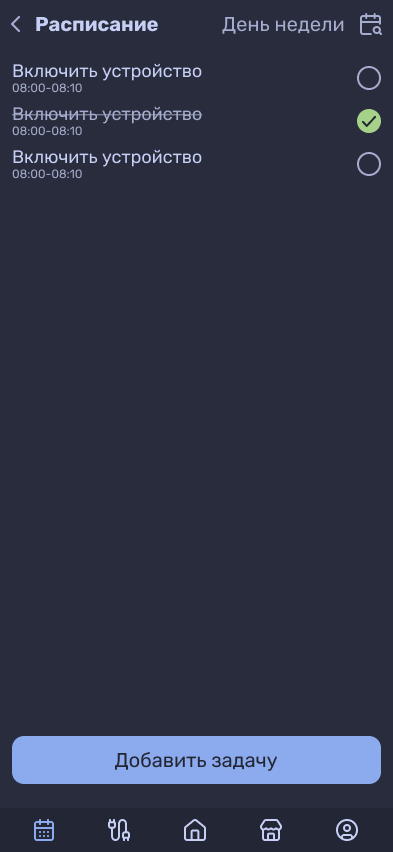
\includegraphics[width=0.425\textwidth]{pics/Calendar Page.png}
  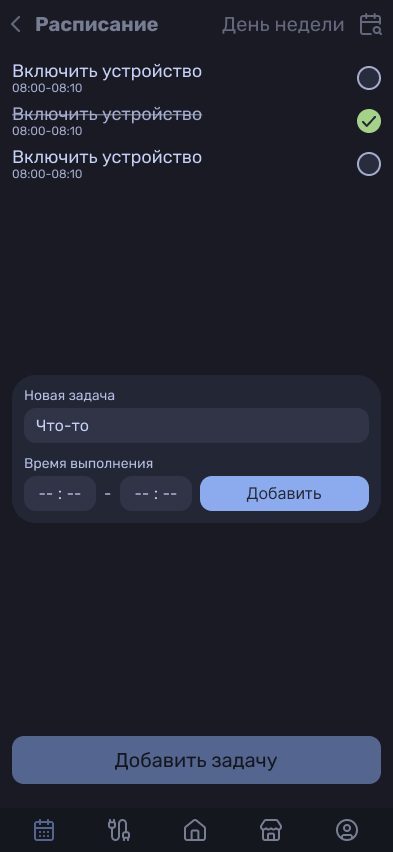
\includegraphics[width=0.425\textwidth]{pics/Calendar Page-1.png}
\end{center}

\end{document}